\documentclass[letterpaper,9pt,twoside,]{pinp}

%% Some pieces required from the pandoc template
\providecommand{\tightlist}{%
  \setlength{\itemsep}{0pt}\setlength{\parskip}{0pt}}

% Use the lineno option to display guide line numbers if required.
% Note that the use of elements such as single-column equations
% may affect the guide line number alignment.

\usepackage[T1]{fontenc}
\usepackage[utf8]{inputenc}
\usepackage{longtable}

% pinp change: the geometry package layout settings need to be set here, not in pinp.cls
\geometry{layoutsize={0.95588\paperwidth,0.98864\paperheight},%
  layouthoffset=0.02206\paperwidth, layoutvoffset=0.00568\paperheight}

\definecolor{pinpblue}{HTML}{185FAF}  % imagecolorpicker on blue for new R logo
\definecolor{pnasbluetext}{RGB}{101,0,0} %



\title{Exploratory Data Analysis (EDA) Project}

\author[CSU, Chico]{Martin Frigaard}

  \affil[a]{California State University, Chico, 400 W 1st St, Chico, CA
95929}

\setcounter{secnumdepth}{0}

% Please give the surname of the lead author for the running footer
\leadauthor{Frigaard}

% Keywords are not mandatory, but authors are strongly encouraged to provide them. If provided, please include two to five keywords, separated by the pipe symbol, e.g:
 \keywords{  EDA |   |  Visualizations  }  

\begin{abstract}
Your first project is an exploratory data analysis (EDA) of a dataset of
your choosing. This document covers set up instructions, functions for
checking the structure of your data, basic summary statistics, and
visualizations.
\end{abstract}

\dates{This version was compiled on \today} 


% initially we use doi so keep for backwards compatibility
% new name is doi_footer
\doifooter{\url{https://mjfrigaard.github.io/csuc-data-journalism/}}

\pinpfootercontents{EDA Project}

\begin{document}

% Optional adjustment to line up main text (after abstract) of first page with line numbers, when using both lineno and twocolumn options.
% You should only change this length when you've finalised the article contents.
\verticaladjustment{-2pt}

\maketitle
\thispagestyle{firststyle}
\ifthenelse{\boolean{shortarticle}}{\ifthenelse{\boolean{singlecolumn}}{\abscontentformatted}{\abscontent}}{}

% If your first paragraph (i.e. with the \dropcap) contains a list environment (quote, quotation, theorem, definition, enumerate, itemize...), the line after the list may have some extra indentation. If this is the case, add \parshape=0 to the end of the list environment.


\hypertarget{introduction}{%
\section{Introduction}\label{introduction}}

This document outlines the requirements for your first project, which is
an exploratory data analysis (EDA) of a dataset (or multiple datasets).

\hypertarget{project-setup}{%
\section{Project setup}\label{project-setup}}

For this assignment, you've been given a dataset (or datasets) and the
EDA template. You should set up your project using the
\href{https://github.com/mjfrigaard/goodenuffR}{\texttt{goodenuffR}
package} package. You can review the slides for getting started with
this package
\href{https://mjfrigaard.github.io/csuc-data-journalism/slides/wk-08.1-intro-to-goodenuffR.html\#1}{here}:

For example, if you've downloaded the \texttt{people-map.csv} data into
your \texttt{Downloads} folder:

\begin{flushleft}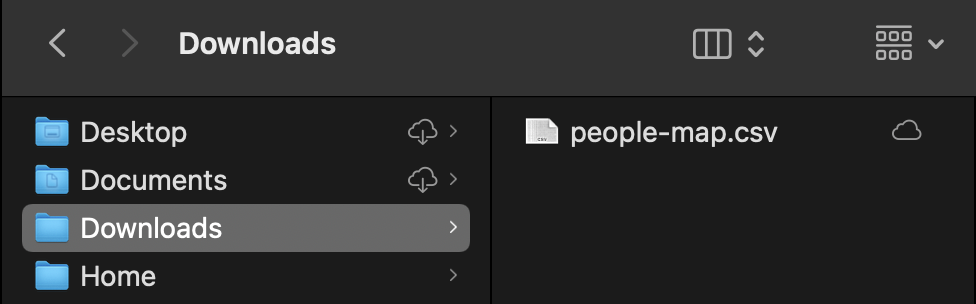
\includegraphics[width=0.5\linewidth]{img/downloads} \end{flushleft}

We're going to create a new project folder using \texttt{goodenuffR}.
Assume I have a folder for the course in \texttt{Documents/} named
\texttt{journalism-303/}:

\begin{flushleft}
\includegraphics[width=0.5\linewidth]{img/course-folder} \end{flushleft}

A folder tree for this type of organization is below:

\begin{Shaded}
\begin{Highlighting}[]
\ExtensionTok{Documents/}
  \KeywordTok{|}\ExtensionTok{{-}{-}}\NormalTok{ journalism{-}303/}
    \KeywordTok{|}\ExtensionTok{{-}{-}}\NormalTok{ exercises/}
    \KeywordTok{|}\ExtensionTok{{-}{-}}\NormalTok{ slides/}
\end{Highlighting}
\end{Shaded}

To create a project folder, I complete the following steps:

\begin{enumerate}
\def\labelenumi{\arabic{enumi}.}
\tightlist
\item
  Use the \texttt{getwd()} function to print my current working
  directory
\end{enumerate}

\begin{Shaded}
\begin{Highlighting}[]
\FunctionTok{getwd}\NormalTok{()}
\CommentTok{\# \textgreater{} "/Users/mjfrigaard"}
\end{Highlighting}
\end{Shaded}

\begin{enumerate}
\def\labelenumi{\arabic{enumi}.}
\setcounter{enumi}{1}
\tightlist
\item
  I want the new project folder to be named \texttt{eda-project/} and to
  be located under the \texttt{Documents/journalism-303/} folder, like
  so:
\end{enumerate}

\begin{Shaded}
\begin{Highlighting}[]
\ExtensionTok{Documents/}
  \KeywordTok{|}\ExtensionTok{{-}{-}}\NormalTok{ journalism{-}303/}
    \KeywordTok{|}\ExtensionTok{{-}{-}}\NormalTok{ exercises/}
    \KeywordTok{|}\ExtensionTok{{-}{-}}\NormalTok{ slides/}
    \KeywordTok{|}\ExtensionTok{{-}{-}}\NormalTok{ eda{-}project/ }\OperatorTok{\textless{}}\NormalTok{{-} new project folder!}
\end{Highlighting}
\end{Shaded}

So in the \texttt{goodenuffR::goodenuff\_project()} function, I enter
the \textbf{name for the new folder as the \texttt{project\_name}
argument}, and the path to \textbf{where I want this folder in the
\texttt{folder\_path} argument.}

\begin{Shaded}
\begin{Highlighting}[]
\NormalTok{goodenuffR}\SpecialCharTok{::}\FunctionTok{goodenuff\_project}\NormalTok{(}\AttributeTok{project\_name =} \StringTok{"eda{-}project"}\NormalTok{, }
    \AttributeTok{folder\_path =} \StringTok{"/Users/mjfrigaard/Documents/journalism{-}303/"}\NormalTok{)}
\end{Highlighting}
\end{Shaded}

When I execute these commands, a new RStudio session will open and I
should see the following folder structure:

\begin{Shaded}
\begin{Highlighting}[]
\ExtensionTok{Documents/}
\KeywordTok{|}\ExtensionTok{{-}{-}journalism{-}303/}
  \KeywordTok{|}\ExtensionTok{{-}{-}}\NormalTok{ eda\_project/}
          \KeywordTok{|}\ExtensionTok{{-}{-}}\NormalTok{ eda\_project.Rproj}
  \KeywordTok{|}\ExtensionTok{{-}{-}}\NormalTok{ exercises/}
  \KeywordTok{|}\ExtensionTok{{-}{-}}\NormalTok{ slides/}
\end{Highlighting}
\end{Shaded}

\begin{flushleft}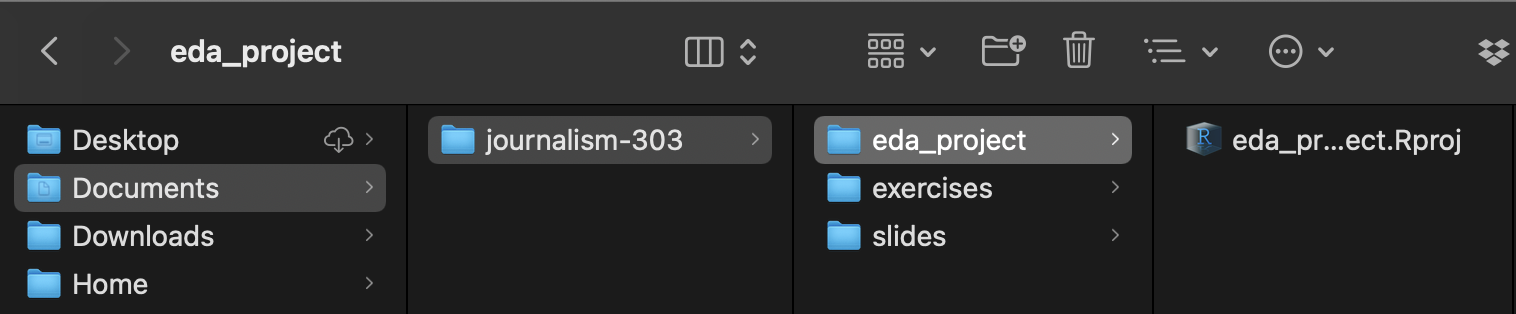
\includegraphics[width=0.7\linewidth]{img/proj-folder} \end{flushleft}

To create the project files, use the
\texttt{goodenuffR::goodenuff\_files()} function. We can enter this into
the console (you should see the following output):

\begin{Shaded}
\begin{Highlighting}[]
\NormalTok{goodenuffR}\SpecialCharTok{::}\FunctionTok{goodenuff\_files}\NormalTok{()}
\CommentTok{\# trying URL \textquotesingle{}https://creativecommons.org/publicdomain/zero/1.0/legalcode.txt\textquotesingle{}     }
\CommentTok{\# downloaded 7048 bytes}
\CommentTok{\# }
\CommentTok{\# trying URL \textquotesingle{}https://raw.githubusercontent.com/rstudio/rmarkdown/main/inst/rmar}
\CommentTok{\# kdown/templates/github\_document/skeleton/skeleton.Rmd\textquotesingle{}}
\CommentTok{\# Content type \textquotesingle{}text/plain; charset=utf{-}8\textquotesingle{} length 691 bytes}
\CommentTok{\# ==================================================}
\CommentTok{\# downloaded 691 bytes}
\end{Highlighting}
\end{Shaded}

This will create the following folders and files:

\begin{flushleft}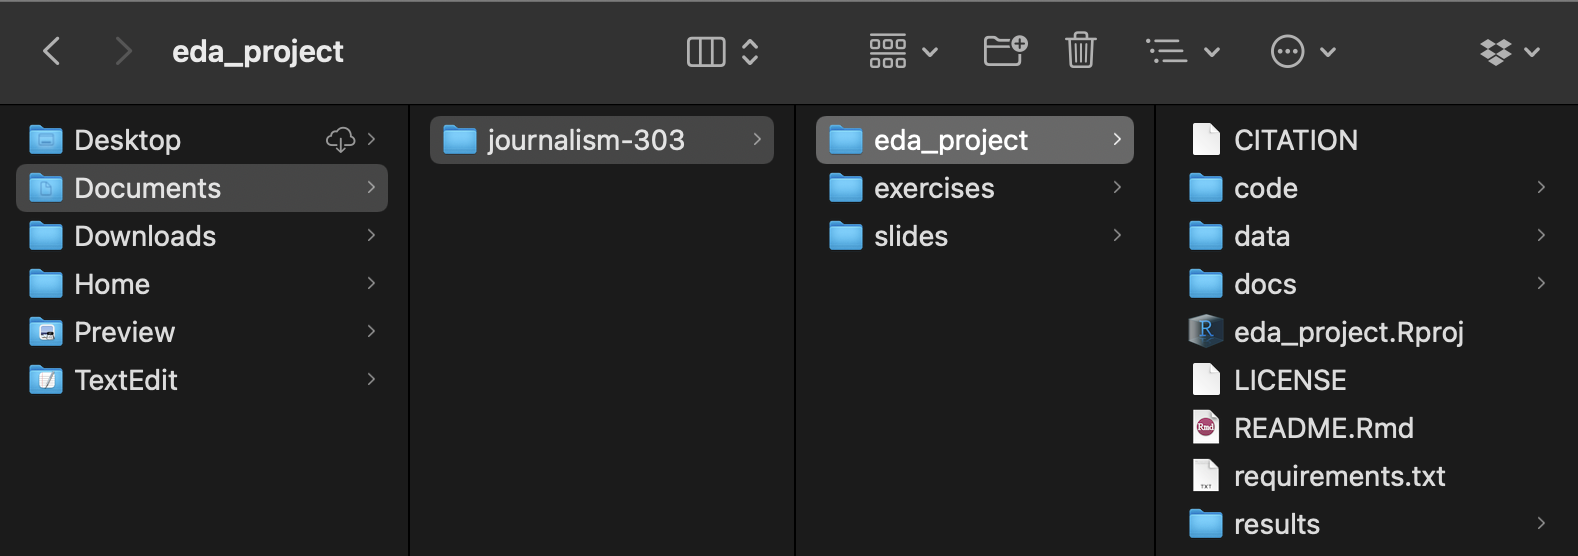
\includegraphics[width=0.8\linewidth]{img/proj-files} \end{flushleft}

And the folder tree below:

\begin{Shaded}
\begin{Highlighting}[]
\ExtensionTok{Documents/}
    \ExtensionTok{journalism{-}303/}
        \KeywordTok{|}\ExtensionTok{{-}{-}}\NormalTok{ eda\_project/}
        \KeywordTok{|}   \KeywordTok{|}\ExtensionTok{{-}{-}}\NormalTok{ CITATION}
        \KeywordTok{|}   \KeywordTok{|}\ExtensionTok{{-}{-}}\NormalTok{ LICENSE}
        \KeywordTok{|}   \KeywordTok{|}\ExtensionTok{{-}{-}}\NormalTok{ README.Rmd}
        \KeywordTok{|}   \KeywordTok{|}\ExtensionTok{{-}{-}}\NormalTok{ code/}
        \KeywordTok{|}   \KeywordTok{|}   \KeywordTok{|}\ExtensionTok{{-}{-}}\NormalTok{ 01{-}import.R}
        \KeywordTok{|}   \KeywordTok{|}   \KeywordTok{|}\ExtensionTok{{-}{-}}\NormalTok{ 02{-}tidy.R}
        \KeywordTok{|}   \KeywordTok{|}   \KeywordTok{|}\ExtensionTok{{-}{-}}\NormalTok{ 03{-}wrangle.R}
        \KeywordTok{|}   \KeywordTok{|}   \KeywordTok{|}\ExtensionTok{{-}{-}}\NormalTok{ 04{-}visualize.R}
        \KeywordTok{|}   \KeywordTok{|}   \KeywordTok{|}\ExtensionTok{{-}{-}}\NormalTok{ 05{-}model.R}
        \KeywordTok{|}   \KeywordTok{|}   \KeywordTok{|}\ExtensionTok{{-}{-}}\NormalTok{ 06{-}communicate.R}
        \KeywordTok{|}   \KeywordTok{|}   \KeywordTok{|}\ExtensionTok{{-}{-}}\NormalTok{ runall.R}
        \KeywordTok{|}   \KeywordTok{|}\ExtensionTok{{-}{-}}\NormalTok{ data/}
        \KeywordTok{|}   \KeywordTok{|}   \KeywordTok{|}\ExtensionTok{{-}{-}}\NormalTok{ README.md}
        \KeywordTok{|}   \KeywordTok{|}   \KeywordTok{|}\ExtensionTok{{-}{-}}\NormalTok{ raw}
        \KeywordTok{|}   \KeywordTok{|}\ExtensionTok{{-}{-}}\NormalTok{ docs/}
        \KeywordTok{|}   \KeywordTok{|}   \KeywordTok{|}\ExtensionTok{{-}{-}}\NormalTok{ changelog.txt}
        \KeywordTok{|}   \KeywordTok{|}   \KeywordTok{|}\ExtensionTok{{-}{-}}\NormalTok{ manuscript.Rmd}
        \KeywordTok{|}   \KeywordTok{|}   \KeywordTok{|}\ExtensionTok{{-}{-}}\NormalTok{ notebook.Rmd}
        \KeywordTok{|}   \KeywordTok{|}\ExtensionTok{{-}{-}}\NormalTok{ eda\_project.Rproj}
        \KeywordTok{|}   \KeywordTok{|}\ExtensionTok{{-}{-}}\NormalTok{ requirements.txt}
        \KeywordTok{|}   \KeywordTok{|}\ExtensionTok{{-}{-}}\NormalTok{ results/}
        \KeywordTok{|}       \KeywordTok{|}\ExtensionTok{{-}{-}}\NormalTok{ figures}
        \KeywordTok{|}       \KeywordTok{|}\ExtensionTok{{-}{-}}\NormalTok{ manuscript}
        \KeywordTok{|}       \KeywordTok{|}\ExtensionTok{{-}{-}}\NormalTok{ tables}
        \KeywordTok{|}\ExtensionTok{{-}{-}}\NormalTok{ exercises/}
        \KeywordTok{|}\ExtensionTok{{-}{-}}\NormalTok{ slides/}
\end{Highlighting}
\end{Shaded}

\hypertarget{outline}{%
\section{Outline}\label{outline}}

After you've set up your project and imported your data into RStudio,
you need to answer the following questions:

\begin{enumerate}
\def\labelenumi{\arabic{enumi}.}
\tightlist
\item
  What are the general characteristics of the dataset?\\
\end{enumerate}

\begin{enumerate}
\def\labelenumi{\alph{enumi}.}
\tightlist
\item
  \emph{How many rows are in the dataset(s)?}\\
\item
  \emph{How many variables are in the dataset(s)?}\\
\end{enumerate}

\begin{enumerate}
\def\labelenumi{\arabic{enumi}.}
\setcounter{enumi}{1}
\tightlist
\item
  What are the variable names?\\
\end{enumerate}

\begin{enumerate}
\def\labelenumi{\alph{enumi}.}
\tightlist
\item
  \emph{Are the names meaningful?}\\
\item
  \emph{Is a data dictionary available (or other info on the
  dataset)?}\\
\item
  \emph{What if the format or type of each variable (i.e.~character,
  numeric, categorical, logical)?}\\
\end{enumerate}

\begin{enumerate}
\def\labelenumi{\arabic{enumi}.}
\setcounter{enumi}{2}
\tightlist
\item
  Information about the variables:\\
\end{enumerate}

\begin{enumerate}
\def\labelenumi{\alph{enumi}.}
\tightlist
\item
  \emph{For categorical/qualitative variables, what values occurs most
  frequently?}\\
\item
  \emph{Are any of the data missing? If so, how much?}\\
\end{enumerate}

\begin{enumerate}
\def\labelenumi{\arabic{enumi}.}
\setcounter{enumi}{3}
\tightlist
\item
  Summary statistics:
\end{enumerate}

\begin{enumerate}
\def\labelenumi{\alph{enumi}.}
\tightlist
\item
  \emph{Calculate the mean, median, standard deviation, minimum, and
  maximum for each numerical variable.}\\
\item
  \emph{Calculate the counts for each level or unique values for each
  character variable.}
\end{enumerate}

\hypertarget{dataset-characteristics}{%
\section{Dataset characteristics}\label{dataset-characteristics}}

We'll use the \texttt{palmerpenguins} data for this example.

\begin{Shaded}
\begin{Highlighting}[]
\CommentTok{\# assign to PenguinsRaw}
\NormalTok{PenguinsRaw }\OtherTok{\textless{}{-}}\NormalTok{ palmerpenguins}\SpecialCharTok{::}\NormalTok{penguins\_raw}
\end{Highlighting}
\end{Shaded}

\hypertarget{dimensions}{%
\subsection{Dimensions}\label{dimensions}}

The functions below give you an idea of the dataset shape.

\begin{Shaded}
\begin{Highlighting}[]
\FunctionTok{nrow}\NormalTok{(PenguinsRaw) }\CommentTok{\# number of rows}
\end{Highlighting}
\end{Shaded}

\begin{ShadedResult}
\begin{verbatim}
#>  [1] 344
\end{verbatim}
\end{ShadedResult}

\begin{Shaded}
\begin{Highlighting}[]
\FunctionTok{ncol}\NormalTok{(PenguinsRaw) }\CommentTok{\# number of columns}
\end{Highlighting}
\end{Shaded}

\begin{ShadedResult}
\begin{verbatim}
#>  [1] 17
\end{verbatim}
\end{ShadedResult}

\begin{Shaded}
\begin{Highlighting}[]
\FunctionTok{dim}\NormalTok{(PenguinsRaw) }\CommentTok{\# dimensions}
\end{Highlighting}
\end{Shaded}

\begin{ShadedResult}
\begin{verbatim}
#>  [1] 344  17
\end{verbatim}
\end{ShadedResult}

For information on the data format, use \texttt{str()} or
\texttt{glimpse()}

\begin{Shaded}
\begin{Highlighting}[]
\FunctionTok{glimpse}\NormalTok{(PenguinsRaw)}
\end{Highlighting}
\end{Shaded}

\begin{ShadedResult}
\begin{verbatim}
#>  Rows: 344
#>  Columns: 17
#>  $ studyName             <chr> "PAL0708", "PAL0708", "PAL07~
#>  $ `Sample Number`       <dbl> 1, 2, 3, 4, 5, 6, 7, 8, 9, 1~
#>  $ Species               <chr> "Adelie Penguin (Pygoscelis ~
#>  $ Region                <chr> "Anvers", "Anvers", "Anvers"~
#>  $ Island                <chr> "Torgersen", "Torgersen", "T~
#>  $ Stage                 <chr> "Adult, 1 Egg Stage", "Adult~
#>  $ `Individual ID`       <chr> "N1A1", "N1A2", "N2A1", "N2A~
#>  $ `Clutch Completion`   <chr> "Yes", "Yes", "Yes", "Yes", ~
#>  $ `Date Egg`            <date> 2007-11-11, 2007-11-11, 200~
#>  $ `Culmen Length (mm)`  <dbl> 39.1, 39.5, 40.3, NA, 36.7, ~
#>  $ `Culmen Depth (mm)`   <dbl> 18.7, 17.4, 18.0, NA, 19.3, ~
#>  $ `Flipper Length (mm)` <dbl> 181, 186, 195, NA, 193, 190,~
#>  $ `Body Mass (g)`       <dbl> 3750, 3800, 3250, NA, 3450, ~
#>  $ Sex                   <chr> "MALE", "FEMALE", "FEMALE", ~
#>  $ `Delta 15 N (o/oo)`   <dbl> NA, 8.94956, 8.36821, NA, 8.~
#>  $ `Delta 13 C (o/oo)`   <dbl> NA, -24.69454, -25.33302, NA~
#>  $ Comments              <chr> "Not enough blood for isotop~
\end{verbatim}
\end{ShadedResult}

\hypertarget{column-names}{%
\section{Column names}\label{column-names}}

We want to standardize the column names so they are easier to program
with.

\begin{Shaded}
\begin{Highlighting}[]
\FunctionTok{library}\NormalTok{(janitor)}
\NormalTok{Penguins }\OtherTok{\textless{}{-}}\NormalTok{ PenguinsRaw }\SpecialCharTok{\%\textgreater{}\%}\NormalTok{ janitor}\SpecialCharTok{::}\FunctionTok{clean\_names}\NormalTok{()}
\FunctionTok{glimpse}\NormalTok{(Penguins)}
\end{Highlighting}
\end{Shaded}

\begin{ShadedResult}
\begin{verbatim}
#>  Rows: 344
#>  Columns: 17
#>  $ study_name        <chr> "PAL0708", "PAL0708", "PAL0708",~
#>  $ sample_number     <dbl> 1, 2, 3, 4, 5, 6, 7, 8, 9, 10, 1~
#>  $ species           <chr> "Adelie Penguin (Pygoscelis adel~
#>  $ region            <chr> "Anvers", "Anvers", "Anvers", "A~
#>  $ island            <chr> "Torgersen", "Torgersen", "Torge~
#>  $ stage             <chr> "Adult, 1 Egg Stage", "Adult, 1 ~
#>  $ individual_id     <chr> "N1A1", "N1A2", "N2A1", "N2A2", ~
#>  $ clutch_completion <chr> "Yes", "Yes", "Yes", "Yes", "Yes~
#>  $ date_egg          <date> 2007-11-11, 2007-11-11, 2007-11~
#>  $ culmen_length_mm  <dbl> 39.1, 39.5, 40.3, NA, 36.7, 39.3~
#>  $ culmen_depth_mm   <dbl> 18.7, 17.4, 18.0, NA, 19.3, 20.6~
#>  $ flipper_length_mm <dbl> 181, 186, 195, NA, 193, 190, 181~
#>  $ body_mass_g       <dbl> 3750, 3800, 3250, NA, 3450, 3650~
#>  $ sex               <chr> "MALE", "FEMALE", "FEMALE", NA, ~
#>  $ delta_15_n_o_oo   <dbl> NA, 8.94956, 8.36821, NA, 8.7665~
#>  $ delta_13_c_o_oo   <dbl> NA, -24.69454, -25.33302, NA, -2~
#>  $ comments          <chr> "Not enough blood for isotopes."~
\end{verbatim}
\end{ShadedResult}

Some of these names are a little long, but we can manually change them
with \texttt{rename()}.

\begin{Shaded}
\begin{Highlighting}[]
\NormalTok{Penguins }\OtherTok{\textless{}{-}}\NormalTok{ Penguins }\SpecialCharTok{\%\textgreater{}\%} 
  \FunctionTok{rename}\NormalTok{(}
    \AttributeTok{study =}\NormalTok{ study\_name,}
    \AttributeTok{sample =}\NormalTok{ sample\_number,}
    \AttributeTok{ind\_id =}\NormalTok{ individual\_id, }
    \AttributeTok{clutch\_cmp =}\NormalTok{ clutch\_completion, }
    \AttributeTok{cul\_lngth =}\NormalTok{ culmen\_length\_mm,}
    \AttributeTok{cul\_dpth =}\NormalTok{ culmen\_depth\_mm, }
    \AttributeTok{flip\_lngth =}\NormalTok{ flipper\_length\_mm, }
    \AttributeTok{body\_mass =}\NormalTok{ body\_mass\_g, }
    \AttributeTok{delta15 =}\NormalTok{ delta\_15\_n\_o\_oo, }
    \AttributeTok{delta13 =}\NormalTok{ delta\_13\_c\_o\_oo}
\NormalTok{  )}
\FunctionTok{glimpse}\NormalTok{(Penguins)}
\end{Highlighting}
\end{Shaded}

\begin{ShadedResult}
\begin{verbatim}
#>  Rows: 344
#>  Columns: 17
#>  $ study      <chr> "PAL0708", "PAL0708", "PAL0708", "PAL07~
#>  $ sample     <dbl> 1, 2, 3, 4, 5, 6, 7, 8, 9, 10, 11, 12, ~
#>  $ species    <chr> "Adelie Penguin (Pygoscelis adeliae)", ~
#>  $ region     <chr> "Anvers", "Anvers", "Anvers", "Anvers",~
#>  $ island     <chr> "Torgersen", "Torgersen", "Torgersen", ~
#>  $ stage      <chr> "Adult, 1 Egg Stage", "Adult, 1 Egg Sta~
#>  $ ind_id     <chr> "N1A1", "N1A2", "N2A1", "N2A2", "N3A1",~
#>  $ clutch_cmp <chr> "Yes", "Yes", "Yes", "Yes", "Yes", "Yes~
#>  $ date_egg   <date> 2007-11-11, 2007-11-11, 2007-11-16, 20~
#>  $ cul_lngth  <dbl> 39.1, 39.5, 40.3, NA, 36.7, 39.3, 38.9,~
#>  $ cul_dpth   <dbl> 18.7, 17.4, 18.0, NA, 19.3, 20.6, 17.8,~
#>  $ flip_lngth <dbl> 181, 186, 195, NA, 193, 190, 181, 195, ~
#>  $ body_mass  <dbl> 3750, 3800, 3250, NA, 3450, 3650, 3625,~
#>  $ sex        <chr> "MALE", "FEMALE", "FEMALE", NA, "FEMALE~
#>  $ delta15    <dbl> NA, 8.94956, 8.36821, NA, 8.76651, 8.66~
#>  $ delta13    <dbl> NA, -24.69454, -25.33302, NA, -25.32426~
#>  $ comments   <chr> "Not enough blood for isotopes.", NA, N~
\end{verbatim}
\end{ShadedResult}

\hypertarget{summary-statistics}{%
\section{Summary statistics}\label{summary-statistics}}

To calculate summary statistics, I recommend using the
\texttt{skimr::skim()} function.

\begin{Shaded}
\begin{Highlighting}[]
\NormalTok{Penguins }\SpecialCharTok{\%\textgreater{}\%} 
  \FunctionTok{skim}\NormalTok{()}
\end{Highlighting}
\end{Shaded}

\begin{longtable}[]{@{}ll@{}}
\caption{Data summary}\tabularnewline
\toprule
\endhead
Name & Piped data \\
Number of rows & 344 \\
Number of columns & 17 \\
\_\_\_\_\_\_\_\_\_\_\_\_\_\_\_\_\_\_\_\_\_\_\_ & \\
Column type frequency: & \\
character & 9 \\
Date & 1 \\
numeric & 7 \\
\_\_\_\_\_\_\_\_\_\_\_\_\_\_\_\_\_\_\_\_\_\_\_\_ & \\
Group variables & None \\
\bottomrule
\end{longtable}

\textbf{Variable type: character}

\begin{longtable}[]{@{}lrrrrrrr@{}}
\toprule
skim\_variable & n\_missing & complete\_rate & min & max & empty &
n\_unique & whitespace \\
\midrule
\endhead
study & 0 & 1.00 & 7 & 7 & 0 & 3 & 0 \\
species & 0 & 1.00 & 33 & 41 & 0 & 3 & 0 \\
region & 0 & 1.00 & 6 & 6 & 0 & 1 & 0 \\
island & 0 & 1.00 & 5 & 9 & 0 & 3 & 0 \\
stage & 0 & 1.00 & 18 & 18 & 0 & 1 & 0 \\
ind\_id & 0 & 1.00 & 4 & 6 & 0 & 190 & 0 \\
clutch\_cmp & 0 & 1.00 & 2 & 3 & 0 & 2 & 0 \\
sex & 11 & 0.97 & 4 & 6 & 0 & 2 & 0 \\
comments & 290 & 0.16 & 18 & 68 & 0 & 10 & 0 \\
\bottomrule
\end{longtable}

\textbf{Variable type: Date}

\begin{longtable}[]{@{}lrrlllr@{}}
\toprule
skim\_variable & n\_missing & complete\_rate & min & max & median &
n\_unique \\
\midrule
\endhead
date\_egg & 0 & 1 & 2007-11-09 & 2009-12-01 & 2008-11-09 & 50 \\
\bottomrule
\end{longtable}

\textbf{Variable type: numeric}

\begin{longtable}[]{@{}lrrrrrrrrr@{}}
\toprule
skim\_variable & n\_missing & complete\_rate & mean & sd & p0 & p25 &
p50 & p75 & p100 \\
\midrule
\endhead
sample & 0 & 1.00 & 63.15 & 40.43 & 1.00 & 29.00 & 58.00 & 95.25 &
152.00 \\
cul\_lngth & 2 & 0.99 & 43.92 & 5.46 & 32.10 & 39.23 & 44.45 & 48.50 &
59.60 \\
cul\_dpth & 2 & 0.99 & 17.15 & 1.97 & 13.10 & 15.60 & 17.30 & 18.70 &
21.50 \\
flip\_lngth & 2 & 0.99 & 200.92 & 14.06 & 172.00 & 190.00 & 197.00 &
213.00 & 231.00 \\
body\_mass & 2 & 0.99 & 4201.75 & 801.95 & 2700.00 & 3550.00 & 4050.00 &
4750.00 & 6300.00 \\
delta15 & 14 & 0.96 & 8.73 & 0.55 & 7.63 & 8.30 & 8.65 & 9.17 & 10.03 \\
delta13 & 13 & 0.96 & -25.69 & 0.79 & -27.02 & -26.32 & -25.83 & -25.06
& -23.79 \\
\bottomrule
\end{longtable}

\hypertarget{skim-output}{%
\subsection{\texorpdfstring{\texttt{skim()}
output}{skim() output}}\label{skim-output}}

The \texttt{factor} variable is qualitative, so the levels are counted
and summarized in the \texttt{n\_unique} and \texttt{top\_counts}. The
\texttt{numeric} variables give us a lot more information, which
includes the \texttt{n\_missing}, \texttt{complete\_rate},
\texttt{mean}, standard deviation (\texttt{sd}), minimum (\texttt{p0}),
25th percentile (\texttt{p25}), median (\texttt{p50}), 75th percentile
(\texttt{p75}), and max (\texttt{p100}).

\hypertarget{exploratory-visualizations}{%
\section{Exploratory visualizations}\label{exploratory-visualizations}}

To complete this project, you'll need to create \textbf{at least one
visualization and explain it's contents.} We've covered how to create
visualizations using \href{https://ggplot2.tidyverse.org/}{ggplot2}, so
feel free to use the code in the exercises or the slides.

\hypertarget{single-variable-graphs}{%
\subsection{Single variable graphs}\label{single-variable-graphs}}

To view the distribution (or `shape') of a variable, you can use
histograms (\texttt{geom\_histogram()}), density plots
(\texttt{geom\_density()}), frequency polygons
(\texttt{geom\_freqpoly()}), or box-plots \texttt{geom\_boxplot()}.

\begin{Shaded}
\begin{Highlighting}[]
\CommentTok{\# label}
\NormalTok{labs\_hist }\OtherTok{\textless{}{-}} \FunctionTok{labs}\NormalTok{(}\AttributeTok{title =} \StringTok{"Histogram of Penguins$flip\_lngth"}\NormalTok{, }
                  \AttributeTok{x =} \StringTok{"Flipper Length"}\NormalTok{)}
\NormalTok{Penguins }\SpecialCharTok{\%\textgreater{}\%} 
  \FunctionTok{ggplot}\NormalTok{(}\FunctionTok{aes}\NormalTok{(}\AttributeTok{x =}\NormalTok{ flip\_lngth)) }\SpecialCharTok{+} 
    \FunctionTok{geom\_histogram}\NormalTok{() }\SpecialCharTok{+} 
\NormalTok{      labs\_hist}
\end{Highlighting}
\end{Shaded}

\begin{center}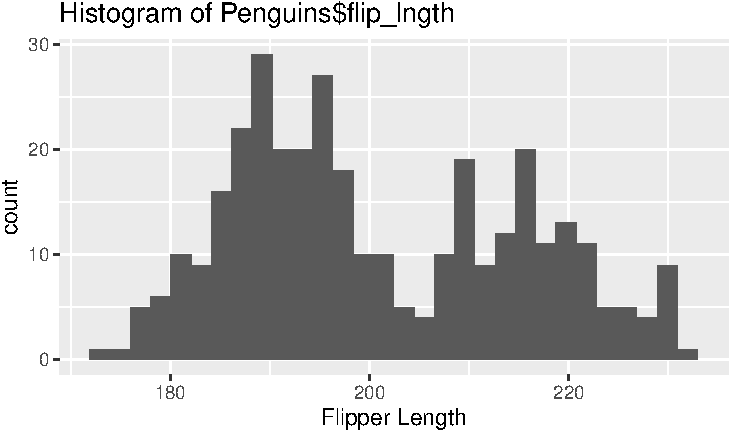
\includegraphics{img/geom_histogram-1} \end{center}

\begin{Shaded}
\begin{Highlighting}[]
\CommentTok{\# label}
\NormalTok{labs\_dens }\OtherTok{\textless{}{-}} \FunctionTok{labs}\NormalTok{(}\AttributeTok{title =} \StringTok{"Density plot of Penguins$flip\_lngth"}\NormalTok{, }
                  \AttributeTok{x =} \StringTok{"Flipper Length"}\NormalTok{)}
\NormalTok{Penguins }\SpecialCharTok{\%\textgreater{}\%} 
  \FunctionTok{ggplot}\NormalTok{(}\FunctionTok{aes}\NormalTok{(}\AttributeTok{x =}\NormalTok{ flip\_lngth)) }\SpecialCharTok{+} 
    \FunctionTok{geom\_density}\NormalTok{() }\SpecialCharTok{+} 
\NormalTok{      labs\_dens}
\end{Highlighting}
\end{Shaded}

\begin{center}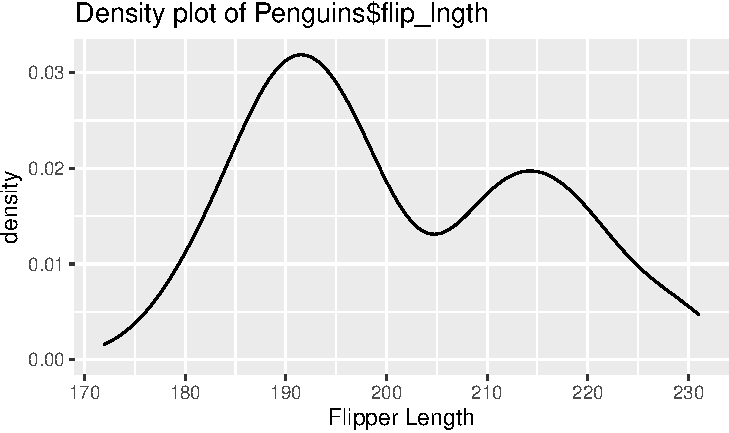
\includegraphics{img/geom_density-1} \end{center}

\begin{Shaded}
\begin{Highlighting}[]
\CommentTok{\# label}
\NormalTok{labs\_freq }\OtherTok{\textless{}{-}} \FunctionTok{labs}\NormalTok{(}\AttributeTok{title =} \StringTok{"Frequency polygon of Penguins$flip\_lngth"}\NormalTok{, }
                  \AttributeTok{x =} \StringTok{"Flipper Length"}\NormalTok{)}
\NormalTok{Penguins }\SpecialCharTok{\%\textgreater{}\%} 
  \FunctionTok{ggplot}\NormalTok{(}\FunctionTok{aes}\NormalTok{(}\AttributeTok{x =}\NormalTok{ flip\_lngth)) }\SpecialCharTok{+} 
    \FunctionTok{geom\_freqpoly}\NormalTok{() }\SpecialCharTok{+} 
\NormalTok{      labs\_freq}
\end{Highlighting}
\end{Shaded}

\begin{center}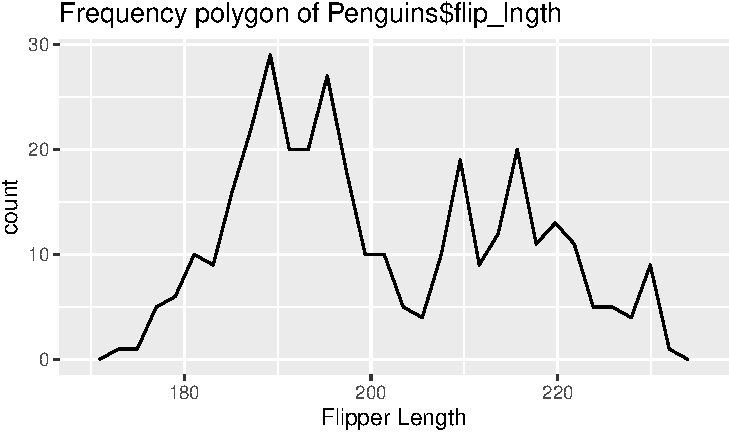
\includegraphics{img/geom_freqpoly-1} \end{center}

\begin{Shaded}
\begin{Highlighting}[]
\CommentTok{\# label}
\NormalTok{labs\_box }\OtherTok{\textless{}{-}} \FunctionTok{labs}\NormalTok{(}\AttributeTok{title =} \StringTok{"Box{-}plot of Penguins$flip\_lngth"}\NormalTok{, }
                  \AttributeTok{x =} \StringTok{"Flipper Length"}\NormalTok{)}
\NormalTok{Penguins }\SpecialCharTok{\%\textgreater{}\%} 
  \FunctionTok{ggplot}\NormalTok{(}\FunctionTok{aes}\NormalTok{(}\AttributeTok{x =}\NormalTok{ flip\_lngth, }
             \AttributeTok{y =} \StringTok{""}\NormalTok{)) }\SpecialCharTok{+} 
  \FunctionTok{geom\_boxplot}\NormalTok{() }\SpecialCharTok{+} 
\NormalTok{  labs\_box}
\end{Highlighting}
\end{Shaded}

\begin{center}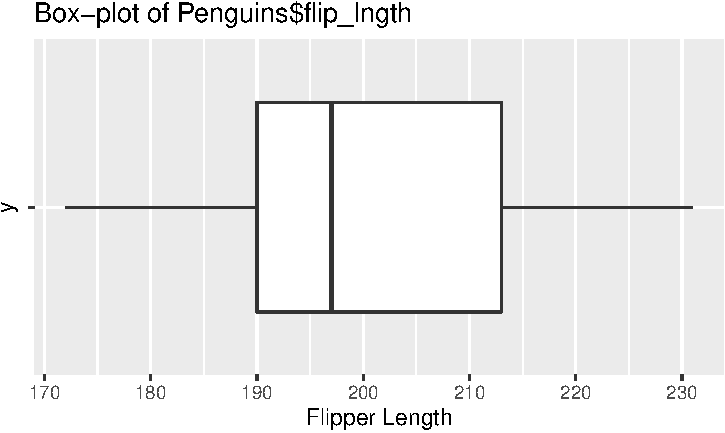
\includegraphics{img/geom_boxplot-1} \end{center}

\hypertarget{relationships-between-variables}{%
\section{Relationships between
variables}\label{relationships-between-variables}}

For exploring relationships between variables, we can use box-plots and
ridgeline plots (from the \texttt{ggridges} package).

\begin{Shaded}
\begin{Highlighting}[]
\NormalTok{labs\_box2 }\OtherTok{\textless{}{-}} \FunctionTok{labs}\NormalTok{(}
     \AttributeTok{title =} \StringTok{"Flipper length by island"}\NormalTok{,}
     \AttributeTok{subtitle =} \StringTok{"source: https://allisonhorst.github.io/palmerpenguins/"}\NormalTok{,}
     \AttributeTok{fill =} \StringTok{"Island"}\NormalTok{,}
     \AttributeTok{x =} \StringTok{"Flipper length"}\NormalTok{,}
     \AttributeTok{y =} \StringTok{"Island"}\NormalTok{)}
\NormalTok{Penguins }\SpecialCharTok{\%\textgreater{}\%}  
  \FunctionTok{ggplot}\NormalTok{() }\SpecialCharTok{+} 
  \FunctionTok{geom\_boxplot}\NormalTok{(}\FunctionTok{aes}\NormalTok{(}\AttributeTok{x =}\NormalTok{ flip\_lngth, }
                      \AttributeTok{y =}\NormalTok{ island, }
                      \AttributeTok{fill =}\NormalTok{ island),}
                      \AttributeTok{alpha =} \DecValTok{1}\SpecialCharTok{/}\DecValTok{5}\NormalTok{) }\SpecialCharTok{+} 
\NormalTok{  labs\_box2}
\end{Highlighting}
\end{Shaded}

\begin{center}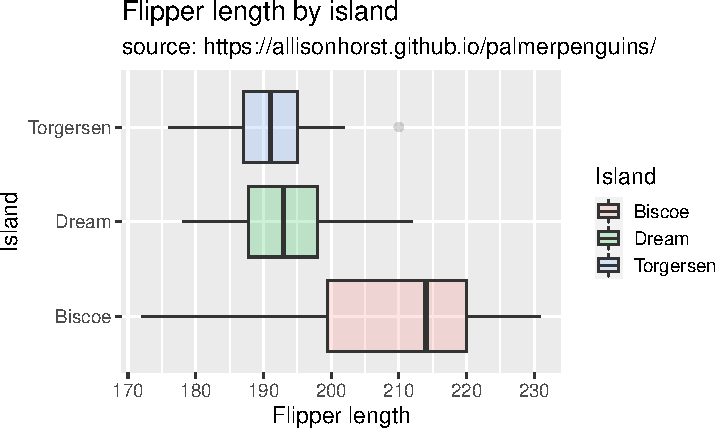
\includegraphics{img/geom_boxplot-2-1} \end{center}

\begin{Shaded}
\begin{Highlighting}[]
\FunctionTok{library}\NormalTok{(ggridges)}
\NormalTok{lab\_ridges }\OtherTok{\textless{}{-}} \FunctionTok{labs}\NormalTok{(}
     \AttributeTok{title =} \StringTok{"Flipper length by island"}\NormalTok{,}
     \AttributeTok{subtitle =} \StringTok{"source: https://allisonhorst.github.io/palmerpenguins/"}\NormalTok{,}
     \AttributeTok{fill =} \StringTok{"Island"}\NormalTok{,}
     \AttributeTok{x =} \StringTok{"Flipper length"}\NormalTok{,}
     \AttributeTok{y =} \StringTok{"Island"}\NormalTok{)}
\NormalTok{Penguins }\SpecialCharTok{\%\textgreater{}\%}  
  \FunctionTok{ggplot}\NormalTok{() }\SpecialCharTok{+} 
  \FunctionTok{geom\_density\_ridges}\NormalTok{(}\FunctionTok{aes}\NormalTok{(}\AttributeTok{x =}\NormalTok{ flip\_lngth, }
                          \AttributeTok{y =}\NormalTok{ island, }
                          \AttributeTok{fill =}\NormalTok{ island), }
                      \AttributeTok{alpha =} \DecValTok{1}\SpecialCharTok{/}\DecValTok{5}\NormalTok{) }\SpecialCharTok{+} 
\NormalTok{  lab\_ridges}
\end{Highlighting}
\end{Shaded}

\begin{center}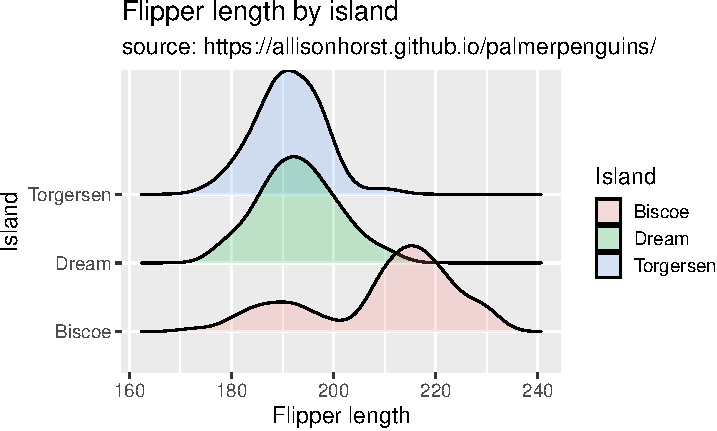
\includegraphics{img/lab_ridges-1} \end{center}

\hypertarget{data-dictionary}{%
\section{Data dictionary}\label{data-dictionary}}

To complete this project, you need to turn in your \texttt{.html} report
and a data dictionary for the dataset which documents each variable and
their contents. For examples, see the example for the
\texttt{palmerpenguins::penguins} data:

\begin{Shaded}
\begin{Highlighting}[]
\NormalTok{??palmerpenguins}\SpecialCharTok{::}\NormalTok{penguins}
\end{Highlighting}
\end{Shaded}

\hypertarget{example-data-dictionary}{%
\subsection{Example data dictionary}\label{example-data-dictionary}}

\begin{quote}
Size measurements for adult foraging penguins near Palmer Station,
Antarctica Description Includes measurements for penguin species, island
in Palmer Archipelago, size (flipper length, body mass, bill
dimensions), and sex. This is a subset of penguins\_raw.
\end{quote}

\begin{quote}
\textbf{Usage}: \texttt{penguins}
\end{quote}

\begin{quote}
\textbf{Format}: A tibble with 344 rows and 8 variables:
\end{quote}

\begin{quote}
\texttt{species}: a factor denoting penguin species (Adélie, Chinstrap
and Gentoo)
\end{quote}

\begin{quote}
\texttt{island}: a factor denoting island in Palmer Archipelago,
Antarctica (Biscoe, Dream or Torgersen)
\end{quote}

\begin{quote}
\texttt{bill\_length\_mm}: a number denoting bill length (millimeters)
\end{quote}

\begin{quote}
\texttt{bill\_depth\_mm}: a number denoting bill depth (millimeters)
\end{quote}

\begin{quote}
\texttt{flipper\_length\_mm}: an integer denoting flipper length
(millimeters)
\end{quote}

\begin{quote}
\texttt{body\_mass\_g}: an integer denoting body mass (grams)
\end{quote}

\begin{quote}
\texttt{sex}: a factor denoting penguin sex (female, male)
\end{quote}

\begin{quote}
\texttt{year}: an integer denoting the study year (2007, 2008, or 2009)
\end{quote}

\begin{quote}
\textbf{Source} Adélie penguins: Palmer Station Antarctica LTER and K.
Gorman. 2020. Structural size measurements and isotopic signatures of
foraging among adult male and female Adélie penguins (Pygoscelis
adeliae) nesting along the Palmer Archipelago near Palmer Station,
2007-2009 ver 5. Environmental Data Initiative
\url{https://doi.org/10.6073/pasta/98b16d7d563f265cb52372c8ca99e60f}
\end{quote}

\begin{quote}
Gentoo penguins: Palmer Station Antarctica LTER and K. Gorman. 2020.
Structural size measurements and isotopic signatures of foraging among
adult male and female Gentoo penguin (Pygoscelis papua) nesting along
the Palmer Archipelago near Palmer Station, 2007-2009 ver 5.
Environmental Data Initiative
\url{https://doi.org/10.6073/pasta/7fca67fb28d56ee2ffa3d9370ebda689}
\end{quote}

\begin{quote}
Chinstrap penguins: Palmer Station Antarctica LTER and K. Gorman. 2020.
Structural size measurements and isotopic signatures of foraging among
adult male and female Chinstrap penguin (Pygoscelis antarcticus) nesting
along the Palmer Archipelago near Palmer Station, 2007-2009 ver 6.
Environmental Data Initiative
\url{https://doi.org/10.6073/pasta/c14dfcfada8ea13a17536e73eb6fbe9e}
\end{quote}

\begin{quote}
Originally published in: Gorman KB, Williams TD, Fraser WR (2014)
Ecological Sexual Dimorphism and Environmental Variability within a
Community of Antarctic Penguins (Genus Pygoscelis). PLoS ONE 9(3):
e90081. \url{doi:10.1371/journal.pone.0090081}
\end{quote}

%\showmatmethods

\pnasbreak 




\end{document}
